\scanpage{25}
% C025-G01 begin
% Complete candidate: \deleted{Soit en effet}
% Ownership: Soit en effet and its one long cancellation only
% Qualification: 
% Hand: his hand
\tikz[x=0.01cm,y=-0.01cm,line cap=round,line join=round,baseline=(base)]{
\coordinate (base) at (0,60);
\useasboundingbox (0,0) rectangle (405,70);
\node[anchor=base west,inner sep=0,outer sep=0] at (0,60) {\rlap{Soit en effet}\phantom{\deleted{Soit en effet}}};
\draw[line width=.6pt] (5,59) .. controls (85,42) and (225,42) .. (400,36);
}
% C025-G01 end
Si on a $U_s\subset
% C025-S01 begin
% Complete candidate: \deleted{E}\Sigma_i^- with short head/retrace
% Complete candidate: \deleted{I}\Sigma_i^- with short head/retrace
% Complete candidate: \deleted{E}\Sigma_{\prime}^- with short head/retrace
% Complete candidate: \deleted{I}\Sigma_{\prime}^- with short head/retrace
% Complete candidate: \deleted{E}\Sigma_i^- with independent upper run
% Complete candidate: \deleted{I}\Sigma_i^- with independent upper run
% Complete candidate: \deleted{E}\Sigma_{\prime}^- with independent upper run
% Complete candidate: \deleted{I}\Sigma_{\prime}^- with independent upper run
% Ownership: Complete overwritten Sigma, old upright, short head, minus and small index; following comma outside
% Qualification: Head/retrace versus independent upper run unresolved; i/prime-like index unresolved. First printed qualifier for recurring detached Sigma heads and undotted short Sigma indices.
% Hand: his hand for body and signs; undetermined hand for independent-upper-run candidate
\unsure{\tikz[x=0.01cm,y=-0.01cm,line cap=round,line join=round,baseline=(base)]{
\coordinate (base) at (0,65);
\useasboundingbox (0,0) rectangle (100,82);
\draw[line width=.85pt] (10,11) .. controls (21,9) and (34,11) .. (46,12);
\draw[line width=.65pt] (11,19) .. controls (20,20) and (34,27) .. (43,32) .. controls (41,39) and (16,54) .. (5,59) .. controls (23,60) and (48,60) .. (61,62) .. controls (65,63) and (65,67) .. (65,71);
\draw[line width=.5pt] (12,20) .. controls (7,22) and (8,26) .. (8,29);
\draw[line width=.5pt] (15,23) .. controls (18,35) and (20,47) .. (19,59);
\draw[line width=.45pt] (14,17) .. controls (27,21) and (35,26) .. (42,31);
\draw[line width=.65pt] (66,10) .. controls (73,9) and (80,11) .. (87,11);
\draw[line width=.7pt] (74,38) .. controls (73,41) and (76,44) .. (77,46);
\node[overlay,anchor=base west,inner sep=0,outer sep=0] at (0,65) {\phantom{$\deleted{\unsure{E|I}}\Sigma_{\unsure{i|\prime}}^-$}};
}}
% C025-S01 end
$, $\overline{U_s}
% C025-G02 begin
% Complete candidate: \deleted{=}\cap
% Complete candidate: \cap with unidentified crossed predecessor
% Complete candidate: \cap with two transverse retraces
% Ownership: The old/current relation only; barred U and following E outside
% Qualification: Two short transverse strokes present; old-equals versus retrace allocation unsettled.
% Hand: his hand
\unsure{\tikz[x=0.01cm,y=-0.01cm,line cap=round,line join=round,baseline=(base)]{
\coordinate (base) at (0,30);
\useasboundingbox (0,0) rectangle (45,40);
\draw[line width=.55pt] (5,18) -- (30,17);
\draw[line width=.55pt] (5,27) -- (29,28);
\draw[line width=.8pt] (11,27) .. controls (23,4) and (34,7) .. (39,31);
\node[overlay,anchor=base west,inner sep=0,outer sep=0] at (0,30) {\phantom{$\deleted{\unsure{=}}\cap$}};
}}
% C025-G02 end
% C025-E01 begin
% Complete candidate: E_i with detached top arm
% Complete candidate: E_j with detached top arm
% Complete candidate: E_i with independent upper curve
% Complete candidate: E_j with independent upper curve
% Ownership: Complete E, detached top curve, index body and its single high point
% Qualification: Index i/j unresolved; upper curve top-arm versus independent-run role unresolved. Point belongs to the qualified index group, no second dot supplied.
% Hand: his hand for E/body; undetermined hand for independent-upper-curve candidate
\unsure{\tikz[x=0.01cm,y=-0.01cm,line cap=round,line join=round,baseline=(base)]{
\coordinate (base) at (0,43);
\useasboundingbox (0,0) rectangle (72,60);
\draw[line width=.4pt] (11,9) .. controls (18,4) and (29,4) .. (37,10);
\draw[line width=.65pt] (5,11) -- (7,36) .. controls (9,39) and (21,39) .. (28,40);
\draw[line width=.6pt] (8,25) -- (27,24);
\fill (57,25) -- (59,24) -- (58,28) -- (56,29) -- cycle;
\draw[line width=.55pt] (48,41) .. controls (51,45) and (51,49) .. (47,51);
\node[overlay,anchor=base west,inner sep=0,outer sep=0] at (0,43) {\phantom{$E_{\unsure{i|j}}$}};
}}
% C025-E01 end
\ne\varnothing$,
% C025-G03 begin
% Complete candidate: \deleted{et si}
% Ownership: et si and its down-right cancellation; alors outside
% Qualification: 
% Hand: his hand
\tikz[x=0.01cm,y=-0.01cm,line cap=round,line join=round,baseline=(base)]{
\coordinate (base) at (0,43);
\useasboundingbox (0,0) rectangle (132,60);
\node[anchor=base west,inner sep=0,outer sep=0] at (0,42) {\rlap{et si}\phantom{\deleted{et si}}};
\draw[line width=.55pt] (4,23) .. controls (30,32) and (87,42) .. (123,50);
}
% C025-G03 end
alors
% C025-G04 begin
% Complete candidate: on a
% Complete candidate: three reduced separate strokes without established lexical reading
% Ownership: Complete proposed on a only; no duplicate printed on a
% Qualification: Whole phrase reading is uncertain; the three shapes are preserved.
% Hand: his hand proposed for phrase; undetermined hand under nonlexical-strokes alternative
\unsure{\tikz[x=0.01cm,y=-0.01cm,line cap=round,line join=round,baseline=(base)]{
\coordinate (base) at (0,19);
\useasboundingbox (0,0) rectangle (145,28);
\fill (6,15) -- (8,13) -- (12,14) -- (8,17) -- (6,19) -- cycle;
\draw[line width=.45pt] (31,16) .. controls (43,14) and (55,9) .. (62,15);
\draw[line width=.55pt] (128,15) .. controls (131,12) and (134,14) .. (137,15);
\node[overlay,anchor=base west,inner sep=0,outer sep=0] at (0,19) {\phantom{\unsure{on a}}};
}}
% C025-G04 end
\[
\begin{aligned}
U_s=X\setminus\mathop{
% C025-G05 begin
% Complete candidate: \rlap{\raisebox{.65ex}{$\scriptstyle-$}}\bigcup
% Complete candidate: \deleted{\bigcap}\bigcup
% Ownership: Operator body, high cross, upper arch and doubled bowl only; limit alpha in K outside
% Qualification: High cross presence firm; complete earlier-intersection/union state remains unresolved.
% Hand: his hand
\unsure{\tikz[x=0.01cm,y=-0.01cm,line cap=round,line join=round,baseline=(base)]{
\coordinate (base) at (0,66);
\useasboundingbox (0,0) rectangle (82,78);
\draw[line width=.65pt] (16,4) .. controls (18,11) and (19,20) .. (20,29) .. controls (22,47) and (24,66) .. (39,68) .. controls (57,70) and (72,48) .. (72,17);
\draw[line width=.7pt] (24,18) .. controls (26,34) and (24,55) .. (35,64) .. controls (47,73) and (68,54) .. (68,22);
\draw[line width=.45pt] (5,17) .. controls (20,5) and (28,16) .. (30,30);
\draw[line width=.65pt] (7,22) -- (52,21);
\draw[line width=.45pt] (69,16) .. controls (75,20) and (76,35) .. (70,42);
\node[overlay,anchor=base west,inner sep=0,outer sep=0] at (0,66) {\phantom{$\unsure{\rlap{\raisebox{.65ex}{$\scriptstyle-$}}\bigcup|\deleted{\bigcap}\bigcup}$}};
}}
% C025-G05 end
}\limits_{\alpha\in K}
% BEGIN A025-S02
% full-scan origin: (966,251); x=.20pt, y=-.20pt; local baseline: (0,81); fixed drawing rectangle: (0,0)--(98,98).
% complete candidates: \widehat{\Sigma}_\alpha^+ with the two locally qualified upper-index traces
% local role/state qualification: Head/body pale junction observed joined. The two small upper-index traces retain attachment, role, hand and surface-origin uncertainty separately.
\begin{tikzpicture}[x=.20pt,y=-.20pt,baseline=(localbase),line cap=round,line join=round]
\path[use as bounding box] (0,0) rectangle (98,98);
\coordinate (localbase) at (0,81);
\node[overlay,anchor=base west,inner sep=0pt,outer sep=0pt] at (0,81) {\phantom{$\widehat{\Sigma}_\alpha^+$}};
\begin{scope}[shift={(-966,-251)}]
\draw[line width=.43pt] (995,270) -- (1012,260) .. controls (1018,265) and (1022,273) .. (1033,273);
\draw[line width=.54pt] (973,291) -- (1021,287);
\draw[line width=.43pt] (975,291) .. controls (988,296) and (1002,302) .. (1007,309) .. controls (1012,316) and (984,325) .. (970,330) .. controls (997,329) and (1019,327) .. (1028,332);
\draw[line width=.52pt] (1047,284) -- (1051,304);
\draw[line width=.50pt] (1039,294) -- (1060,294);
\draw[line width=.45pt] (1047,337) .. controls (1043,326) and (1030,321) .. (1030,333) .. controls (1030,349) and (1043,342) .. (1048,330) .. controls (1051,324) and (1052,319) .. (1053,314);
\draw[line width=.51pt] (1042,331) .. controls (1046,337) and (1050,341) .. (1057,339);
% BEGIN A025-M01
% nested full-scan origin (1041,306), local baseline (0,0), base-west zero-separation anchor; owns two upper-index traces only.
\node[anchor=base west,inner sep=0pt,outer sep=0pt] at (1041,306) {\unsure{\begin{tikzpicture}[x=.20pt,y=-.20pt,baseline=(markbase)]
\path[use as bounding box] (0,0) rectangle (10,15);\coordinate (markbase) at (0,0);
\draw[gray,line width=.21pt] (1,2) -- (3,3);
\fill (3,9) -- (6,8) -- (8,11) -- (5,14) -- cycle;
\end{tikzpicture}}};
% END A025-M01
\end{scope}
\end{tikzpicture}
% END A025-S02
&\qquad\text{
% C025-G06 begin
% Complete candidate: où
% Complete candidate: ou with separate upper stroke
% Ownership: Complete reduced où including its high stroke; i in K outside
% Qualification: Word and raised-stroke attachment remain qualified.
% Hand: his hand for proposed word; undetermined hand for independent-upper-stroke alternative
\unsure{\tikz[x=0.01cm,y=-0.01cm,line cap=round,line join=round,baseline=(base)]{
\coordinate (base) at (0,25);
\useasboundingbox (0,0) rectangle (66,32);
\fill (5,25) -- (9,20) -- (12,21) -- (10,24) -- cycle;
\draw[line width=.5pt] (23,25) .. controls (32,22) and (42,23) .. (49,24);
\draw[line width=.55pt] (39,7) -- (41,12);
\node[overlay,anchor=base west,inner sep=0,outer sep=0] at (0,25) {\phantom{\unsure{où}}};
}}
% C025-G06 end
}\quad i\in K\subset I\\
&\forall\alpha\in K\qquad
% C025-S03 begin
% Complete candidate: $\Sigma_\alpha^+$
% Ownership: Complete condition Sigma with its joined head, alpha and plus
% Qualification: Head/body join seen locally; no separate head-role uncertainty added.
% Hand: his hand
\tikz[x=0.01cm,y=-0.01cm,line cap=round,line join=round,baseline=(base)]{
\coordinate (base) at (0,40);
\useasboundingbox (0,0) rectangle (100,56);
\draw[line width=.5pt] (10,12) -- (59,8);
\draw[line width=.5pt] (10,12) .. controls (52,22) and (50,23) .. (7,40) -- (57,40);
\draw[line width=.6pt] (76,7) -- (78,18);
\draw[line width=.6pt] (69,12) -- (85,11);
\draw[line width=.55pt] (75,38) .. controls (66,51) and (59,48) .. (60,45) .. controls (63,42) and (76,46) .. (84,47);
\node[overlay,anchor=base west,inner sep=0,outer sep=0] at (0,40) {\phantom{$\Sigma_\alpha^+$}};
}
% C025-S03 end
\in\pi_0(X\setminus
% C025-E02 begin
% Complete candidate: E_\alpha with detached top arm
% Complete candidate: E_\alpha with independent upper run
% Ownership: Complete E_alpha in pi0 argument, all three arms and alpha
% Qualification: Local top-arm/independent-run alternative retained under first E qualifier at E01.
% Hand: his hand for E; undetermined hand for independent-upper-run alternative
\unsure{\tikz[x=0.01cm,y=-0.01cm,line cap=round,line join=round,baseline=(base)]{
\coordinate (base) at (0,39);
\useasboundingbox (0,0) rectangle (59,48);
\draw[line width=.45pt] (8,8) .. controls (15,6) and (22,8) .. (28,8);
\draw[line width=.5pt] (3,8) -- (2,34) -- (23,34);
\draw[line width=.5pt] (4,22) -- (22,22);
\draw[line width=.5pt] (48,28) .. controls (40,43) and (31,41) .. (31,36) .. controls (33,31) and (41,36) .. (49,40);
\node[overlay,anchor=base west,inner sep=0,outer sep=0] at (0,39) {\phantom{$E_\alpha$}};
}}
% C025-E02 end
)\quad\text{
% C025-G07 begin
% Complete candidate: \deleted{les}
% Complete candidate: \deleted{K}
% Complete candidate: \deleted{tel}
% Ownership: Entire crossed endpoint cluster; no separate comma
% Qualification: Letter sequence remains obscured by crossing; H tel preserved as a complete alternative.
% Hand: his hand
\unsure{\tikz[x=0.01cm,y=-0.01cm,line cap=round,line join=round,baseline=(base)]{
\coordinate (base) at (0,47);
\useasboundingbox (0,0) rectangle (72,62);
\draw[line width=.5pt] (12,5) -- (14,46) .. controls (20,44) and (25,38) .. (30,33);
\draw[line width=.5pt] (5,25) -- (36,9) .. controls (36,18) and (25,23) .. (19,30);
\draw[line width=.55pt] (19,30) .. controls (28,37) and (35,37) .. (41,25);
\draw[line width=.55pt] (54,22) .. controls (49,29) and (49,37) .. (48,43);
\draw[line width=.6pt] (23,35) -- (68,34);
\node[overlay,anchor=base west,inner sep=0,outer sep=0] at (0,47) {\phantom{\deleted{\unsure{les|K|tel}}}};
}}
% C025-G07 end
}\\
&
% C025-G08 begin
% Complete candidate: \deleted{U\Sigma}
% Complete candidate: \deleted{\bigcup\Sigma}
% Complete candidate: \deleted{U}
% Complete candidate: U\Sigma
% Complete candidate: \text{et}
% Ownership: Entire pre-les cluster only; live les is outside
% Qualification: Original three cancelled candidates retained; live U Sigma and live et remain whole-state alternatives because no independent strike is isolated.
% Hand: his hand
\unsure{\tikz[x=0.01cm,y=-0.01cm,line cap=round,line join=round,baseline=(base)]{
\coordinate (base) at (0,63);
\useasboundingbox (0,0) rectangle (56,79);
\draw[line width=.45pt] (6,13) .. controls (7,31) and (5,56) .. (17,62) .. controls (32,73) and (46,47) .. (45,10);
\draw[line width=.5pt] (13,25) -- (44,14) -- (26,40) -- (45,39);
\draw[line width=.55pt] (32,62) .. controls (30,75) and (41,73) .. (47,65);
\node[overlay,anchor=base west,inner sep=0,outer sep=0] at (0,63) {\phantom{$\deleted{\unsure{U\Sigma|\bigcup\Sigma|U}}$}};
}}
% C025-G08 end
\ \text{les }
% C025-S04 begin
% Complete candidate: \Sigma_\alpha^+ with detached head/retrace
% Complete candidate: \Sigma_\alpha^+ with independent upper run
% Ownership: Complete disjointness Sigma, head, plus and alpha joined into foot
% Qualification: Local role retained under S01 first qualifier; joined foot/alpha stroke occurs once.
% Hand: his hand for body; undetermined hand for independent-upper-run candidate
\unsure{\tikz[x=0.01cm,y=-0.01cm,line cap=round,line join=round,baseline=(base)]{
\coordinate (base) at (0,39);
\useasboundingbox (0,0) rectangle (77,54);
\draw[line width=.5pt] (13,7) -- (37,8);
\draw[line width=.5pt] (8,15) .. controls (36,18) and (42,15) .. (6,36) .. controls (17,39) and (30,38) .. (40,36) .. controls (49,31) and (51,35) .. (48,40) .. controls (41,48) and (37,42) .. (42,40) .. controls (48,39) and (56,43) .. (58,44);
\draw[line width=.55pt] (58,7) -- (60,20);
\draw[line width=.55pt] (48,11) -- (64,10);
\node[overlay,anchor=base west,inner sep=0,outer sep=0] at (0,39) {\phantom{$\Sigma_\alpha^+$}};
}}
% C025-S04 end
\ \text{mut\textsuperscript{t}. disjoints}
\end{aligned}
\]
Il faut voir que
% BEGIN A025-G09
% full-scan origin: (874,478); x=.20pt, y=-.20pt; local baseline: (0,139); fixed drawing rectangle: (0,0)--(194,162).
% complete candidates: \deleted{K}\inserted{K\setminus\{i\}} with long run acting as guide ; \deleted{K}\inserted{K\setminus\{i\}} with long run acting as strike
% local role/state qualification: Words/state firm; long-run role remains unresolved locally, with source-positioned curved geometry.
\begin{tikzpicture}[x=.20pt,y=-.20pt,baseline=(localbase),line cap=round,line join=round]
\path[use as bounding box] (0,0) rectangle (194,162);
\coordinate (localbase) at (0,139);
\begin{scope}[shift={(-874,-478)}]
\node[anchor=base west,inner sep=0pt,outer sep=0pt] at (880,543) {$\inserted{K\setminus\{i\}}$};
\node[overlay,anchor=base west,inner sep=0pt,outer sep=0pt] at (952,615) {\phantom{$\deleted{K}$}};
\draw[line width=.45pt] (959,552) -- (973,621);
\draw[line width=.45pt] (963,590) -- (1000,564);
\draw[line width=.57pt] (969,597) -- (1000,613);
\draw[line width=.50pt] (979,548) .. controls (991,552) and (1003,540) .. (988,555) -- (962,573) .. controls (979,571) and (996,559) .. (1002,563) .. controls (1018,570) and (977,590) .. (986,600) .. controls (1011,593) and (992,619) .. (978,635);
% BEGIN A025-M02
% long guide/strike: full-scan origin (920,526), local baseline (0,0), base-west zero separation.
\node[anchor=base west,inner sep=0pt,outer sep=0pt] at (920,526) {\unsure{\begin{tikzpicture}[x=.20pt,y=-.20pt,baseline=(guidebase)]
\path[use as bounding box] (0,0) rectangle (145,101);\coordinate (guidebase) at (0,0);
\draw[line width=.28pt] (5,97) .. controls (-2,78) and (19,48) .. (42,42) .. controls (74,32) and (111,20) .. (141,6) .. controls (144,4) and (140,2) .. (136,3);
\end{tikzpicture}}};
% END A025-M02
\end{scope}
\end{tikzpicture}
% END A025-G09
et les $
% C025-S05 begin
% Complete candidate: \Sigma_\alpha^+ with detached head/retrace
% Complete candidate: \Sigma_\alpha^+ with independent upper run
% Ownership: Complete prose Sigma; following parenthetical outside
% Qualification: Local role retained under S01 first qualifier.
% Hand: his hand for body; undetermined hand for independent-upper-run candidate
\unsure{\tikz[x=0.01cm,y=-0.01cm,line cap=round,line join=round,baseline=(base)]{
\coordinate (base) at (0,47);
\useasboundingbox (0,0) rectangle (88,65);
\draw[line width=.45pt] (9,8) -- (49,9);
\draw[line width=.45pt] (13,18) .. controls (53,24) and (40,28) .. (5,46) -- (40,46);
\draw[line width=.5pt] (67,9) -- (69,22);
\draw[line width=.5pt] (59,15) -- (75,15);
\draw[line width=.5pt] (65,43) .. controls (57,57) and (44,56) .. (45,51) .. controls (48,46) and (61,53) .. (69,56);
\node[overlay,anchor=base west,inner sep=0,outer sep=0] at (0,47) {\phantom{$\Sigma_\alpha^+$}};
}}
% C025-S05 end
$ $(\alpha\in K\setminus\{i\})$ sont \unsure{determinés|determines} en termes de $i$ et de $
% C025-S06 begin
% Complete candidate: \Sigma_i^+ with detached head/retrace
% Complete candidate: \Sigma_{\prime}^+ with detached head/retrace
% Complete candidate: \Sigma_i^+ with independent upper run
% Complete candidate: \Sigma_{\prime}^+ with independent upper run
% Ownership: Complete lower first Sigma, interrupted head entrance, body, plus and short index; i.e. outside
% Qualification: Local head and i/prime alternatives retained under first printed S01 qualifier.
% Hand: his hand for body; undetermined hand for independent-upper-run candidate
\unsure{\tikz[x=0.01cm,y=-0.01cm,line cap=round,line join=round,baseline=(base)]{
\coordinate (base) at (0,64);
\useasboundingbox (0,0) rectangle (110,78);
\draw[line width=.3pt] (4,17) -- (5,17);
\draw[line width=.4pt] (9,16) -- (62,8);
\draw[line width=.5pt] (17,23) .. controls (78,25) and (65,35) .. (5,68) .. controls (33,65) and (57,58) .. (76,56) -- (78,64);
\draw[line width=.6pt] (92,8) -- (95,22);
\draw[line width=.6pt] (84,14) -- (102,14);
\draw[line width=.55pt] (78,36) -- (82,39);
\node[overlay,anchor=base west,inner sep=0,outer sep=0] at (0,64) {\phantom{$\Sigma_i^+$}};
}}
% C025-S06 end
$ i.e. $
% C025-S07 begin
% Complete candidate: \Sigma_i^- with detached head/retrace
% Complete candidate: \Sigma_{\prime}^- with detached head/retrace
% Complete candidate: \Sigma_i^- with independent upper run
% Complete candidate: \Sigma_{\prime}^- with independent upper run
% Ownership: Complete lower second Sigma, head, minus and short index; following point outside
% Qualification: Local head and i/prime alternatives retained under first printed S01 qualifier.
% Hand: his hand for body; undetermined hand for independent-upper-run candidate
\unsure{\tikz[x=0.01cm,y=-0.01cm,line cap=round,line join=round,baseline=(base)]{
\coordinate (base) at (0,52);
\useasboundingbox (0,0) rectangle (101,69);
\draw[line width=.4pt] (7,15) -- (45,11);
\draw[line width=.45pt] (6,27) .. controls (64,29) and (41,39) .. (13,53) .. controls (39,48) and (54,47) .. (64,57);
\draw[line width=.55pt] (70,8) -- (91,8);
\draw[line width=.55pt] (66,43) -- (67,47);
\node[overlay,anchor=base west,inner sep=0,outer sep=0] at (0,52) {\phantom{$\Sigma_i^-$}};
}}
% C025-S07 end
$. Je dis $
% BEGIN B025-G09
% proposal: \text{que}
% qualification: Only the small point beside q has unresolved role, hand, attachment and surface origin; que itself is firm.
% complete candidates: que with an unassigned small point beside its q descender
% ownership: Complete final que, its long q descender, and one separate small point at its right. Je dis remains outside; no additional que or point is printed.
\mathord{\unsure{\begin{tikzpicture}[x=0.018em,y=-0.018em,baseline=(base),line cap=round,line join=round]
\path[use as bounding box] (0,0) rectangle (108,113);
\coordinate (base) at (0,30);
\begin{scope}[shift={(-1050,-798)}]
\node[overlay,anchor=base west,inner sep=0pt,outer sep=0pt] at (1050,828) {$\phantom{\text{que}}$};
\draw[line width=.025em] (1063,811) .. controls (1052,802) and (1052,822) .. (1070,823) .. controls (1082,822) and (1086,818) .. (1088,809);
\draw[line width=.025em] (1068,809) .. controls (1075,817) and (1076,849) .. (1079,875) .. controls (1085,902) and (1083,906) .. (1072,903);
\draw[line width=.026em] (1088,809) .. controls (1098,820) and (1116,817) .. (1118,805) .. controls (1124,813) and (1138,811) .. (1147,813) .. controls (1152,814) and (1150,820) .. (1148,821);
\fill (1094,841) -- (1096,840) -- (1096,843) -- cycle;
\end{scope}
\end{tikzpicture}}}
% END B025-G09
$
\[
K\setminus\{i\}=
% BEGIN B025-G08
% proposal: \bigl\{
% ownership: Only the final set left brace, upper and lower arms meeting at the left cusp; alpha and condition follow outside.
\mathord{\begin{tikzpicture}[x=0.018em,y=-0.018em,baseline=(base),line cap=round,line join=round]
\path[use as bounding box] (0,0) rectangle (40,118);
\coordinate (base) at (0,64);
\begin{scope}[shift={(-758,-917)}]
\node[overlay,anchor=base west,inner sep=0pt,outer sep=0pt] at (758,981) {$\phantom{\bigl\{}$};
\draw[line width=.021em] (776,925) .. controls (777,944) and (780,963) .. (779,973) .. controls (775,979) and (769,974) .. (764,974);
\draw[line width=.030em] (764,974) .. controls (783,975) and (781,1006) .. (785,1024) .. controls (790,1032) and (793,1030) .. (795,1031);
\end{scope}
\end{tikzpicture}}
% END B025-G08
\alpha\in I\mid E_\alpha\subset
% BEGIN A025-S08
% full-scan origin: (1169,900); x=.20pt, y=-.20pt; local baseline: (0,55); fixed drawing rectangle: (0,0)--(103,65).
% local role/state qualification: Faint joined head/body junction; alpha and minus firm. No correction to index.
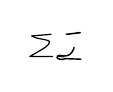
\begin{tikzpicture}[x=.20pt,y=-.20pt,baseline=(localbase),line cap=round,line join=round]
\path[use as bounding box] (0,0) rectangle (103,65);
\coordinate (localbase) at (0,55);
\node[overlay,anchor=base west,inner sep=0pt,outer sep=0pt] at (0,55) {\phantom{$\Sigma_\alpha^-$}};
\begin{scope}[shift={(-1169,-900)}]
\draw[line width=.45pt] (1176,915) -- (1211,912);
\draw[line width=.43pt] (1178,915) .. controls (1183,921) and (1204,920) .. (1208,925) .. controls (1212,932) and (1184,945) .. (1173,952) -- (1214,952);
\draw[line width=.57pt] (1239,912) -- (1264,909);
\draw[line width=.51pt] (1253,936) .. controls (1249,948) and (1243,952) .. (1233,951) .. controls (1215,946) and (1220,962) .. (1238,956) -- (1265,957);
\draw[line width=.35pt] (1224,952) -- (1235,953);
\end{scope}
\end{tikzpicture}
% END A025-S08
\]
% Lower-sheet detached marks, in their own source positions; no lexical role assigned.
\figure{\begin{tikzpicture}[x=0.01em,y=-0.01em]
\path[use as bounding box] (0,0) rectangle (1685,1261);
\node[anchor=base west,inner sep=0pt,outer sep=0pt] at (448,252) {$
% BEGIN B025-M01
% proposal: 
% qualification: Faint curved surface trace, no character assigned; role, hand and surface origin undetermined.
% ownership: Faint upper curve, pale middle continuation, lower diagonal/foot and detached left foot run.
\mathord{\unsure{\begin{tikzpicture}[x=0.01em,y=-0.01em,baseline=(base),line cap=round,line join=round]
\path[use as bounding box] (0,0) rectangle (38,44);
\coordinate (base) at (0,44);
\begin{scope}[shift={(-448,-1308)}]
\draw[line width=.013em,gray] (471,1312) .. controls (477,1315) and (480,1323) .. (480,1333);
\draw[line width=.009em,gray] (480,1333) -- (480,1338);
\draw[line width=.012em,gray] (479,1340) -- (471,1347) -- (460,1347);
\draw[line width=.007em,gray] (456,1347) -- (450,1346);
\end{scope}
\end{tikzpicture}}}
% END B025-M01
$};
\node[anchor=base west,inner sep=0pt,outer sep=0pt] at (1592,630) {$
% BEGIN B025-M02
% proposal: 
% qualification: Two dark diagonal points; character, role, hand and surface origin undetermined.
% ownership: Both isolated lower-right points, with no colon or other character supplied.
\mathord{\unsure{\begin{tikzpicture}[x=0.01em,y=-0.01em,baseline=(base),line cap=round,line join=round]
\path[use as bounding box] (0,0) rectangle (14,17);
\coordinate (base) at (0,17);
\begin{scope}[shift={(-1592,-1713)}]
\fill (1600,1718) ellipse [x radius=1.4,y radius=1.8];
\fill (1595,1725) ellipse [x radius=1.7,y radius=1.6];
\end{scope}
\end{tikzpicture}}}
% END B025-M02
$};
\end{tikzpicture}}
% archive sheet number: 24
